% !TEX root = ../Ausarbeitung.tex
\section{Evolutionary Algorithms}
\label{sec:ea}
Evolutionary algorithms are inspired by nature and evolution.
They try to approximate a solution following the principle of survival of the fittest.
In fact, an evolutionary algorithm models a population consisting of several individuals performing a task, such as an optimization problem, and are evaluated by a fitness function.
One of these populations is called a generation.
The elite of each generation, i.e. the individuals performing best according to their fitness, is then selected to evolve the next generation.
This allows the population to evolve towards a solution.
The evolution of a population corresponds to the mutation of individuals.
The evolution process is depicted in \autoref{fig:ea}.

\begin{figure}[h]
\centering
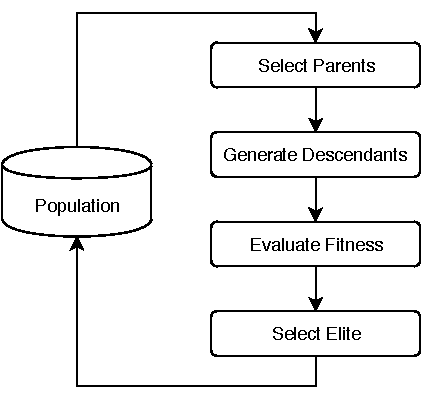
\includegraphics[width=.7\columnwidth]{figures/ea_fig.pdf}
\caption{An illustration of an evolutionary algorithm learning.}
\label{fig:ea}
\end{figure}

To mutate a population, the crossover strategy can be applied.
Crossover is used to generate new offspring by combining genetic information of two parents.
One way to combine their genetic information is single-point crossover.
A point is randomly picked on the genetic sequence, where it is separated at the same point of both parents.
The second part, i.e. the tail, is then swapped between the parents.
Hence, each parent has its own genetic information until the chosen point, following by the genetic sequence of the other parent.
To apply more variety into the recombination of the genetic information k-point crossover can be applied.
Instead of only one point, more such random points are picked in the sequence, at which alternately information is swapped between the parents.

As individuals are evolving over generations, they may improve their fitness and thus optimize a solution for the task.
Their genetic information can therefore be parameters to solve a problem.
Overall, there is no specific or correct parameter assumption needed for initialization, as they will be approximated by evolving over generations.
